\section{Feature Model}\label{ch:Feature Model}

\begin{figure}[h]
    \centering
    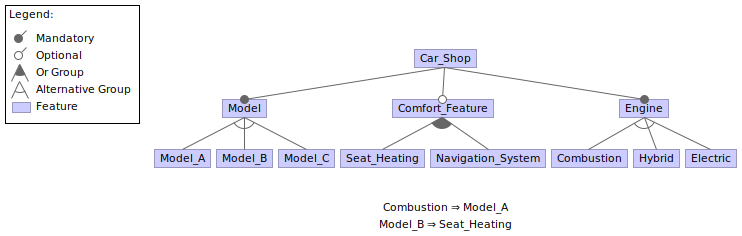
\includegraphics[scale=0.6]{gfx/Car_Shop.png}
    \caption{A feature model of a car dealership}
    \label{fig:car}
\end{figure}

A configurable system often contains numerous features, all of which may interact with one each other or have different dependencies.
To keep track of the system, we introduce feature model \cite{Feature-Oriented-Software-Product-Lines-Feature-models}. An example
of a feature model for a car dealership can be found in \ref{fig:car}

A feature model is essentially a tree that models a configurable system, where each node in that tree represent a specific feature, while the root
represent the system itself. When a feature is selected, it implies that also the parent of that features must also be selected as well, the further
down the tree we go, the more specific features become. In \ref{fig:car} we see Engine is a feature whose children a concrete types
of engines, in particular Combustion, Hybrid and Electric.

Each feature can contain a graphical notation indicating whether the feature is mandatory or optional, if the feature is mandatory it is 
indicated with a black bubble, and if it is optional it is displayed with an empty bubble, in \ref{fig:car} we can see that Engine and
Model are mandatory features, which make sense since both are necessary for any car, but Comfort\_Feature a optional since they are not
necessary for a car to function.

In addition to mandatory and optional features, there are also alternative and choice groups. A parent can have one of these groups, an alternative group
is marked with an empty half circle and an optional group with a filled circle. When a selection group is used, one feature needs to be selected, but
others can be selected as well, a choice group corresponds to the logical or operator. In an alternative group, only one feature can be
selected, if more than one feature is selected the configuration is invalid. In \ref{fig:car} we see that Engine has a alternative group, which makes sense
since each car can only contain one Engine, where it makes sense that Comfort\_Feature contains a choice group, you can have a navigation system
and seat heating in a car without conflict.

In addition, a feature model may contain various constraints that need to be satisfied, these constraints are defined as boolean 
algebra. In \ref{fig:car} we see that there are two constraints, $Combustion \implies Model\_A$ and 
$Model\_B \implies Seat\_Heating$, the reasons for such constraints could be that Model\_B is a luxury model where it only gets shipped
with seat heating.

Any feature model can also be translated into compositional logic \cite*{Feature-Oriented-Software-Product-Lines-Feature-models}, therefore a
configuration of features is valid only iff it satisfies the propositional logic. We can therefore use a feature model to check wheter a 
configuration is valid, which is particularly useful if we want to sample or enumerate all valid configurations. 